\section{Problem Definition}
\begin{figure}
    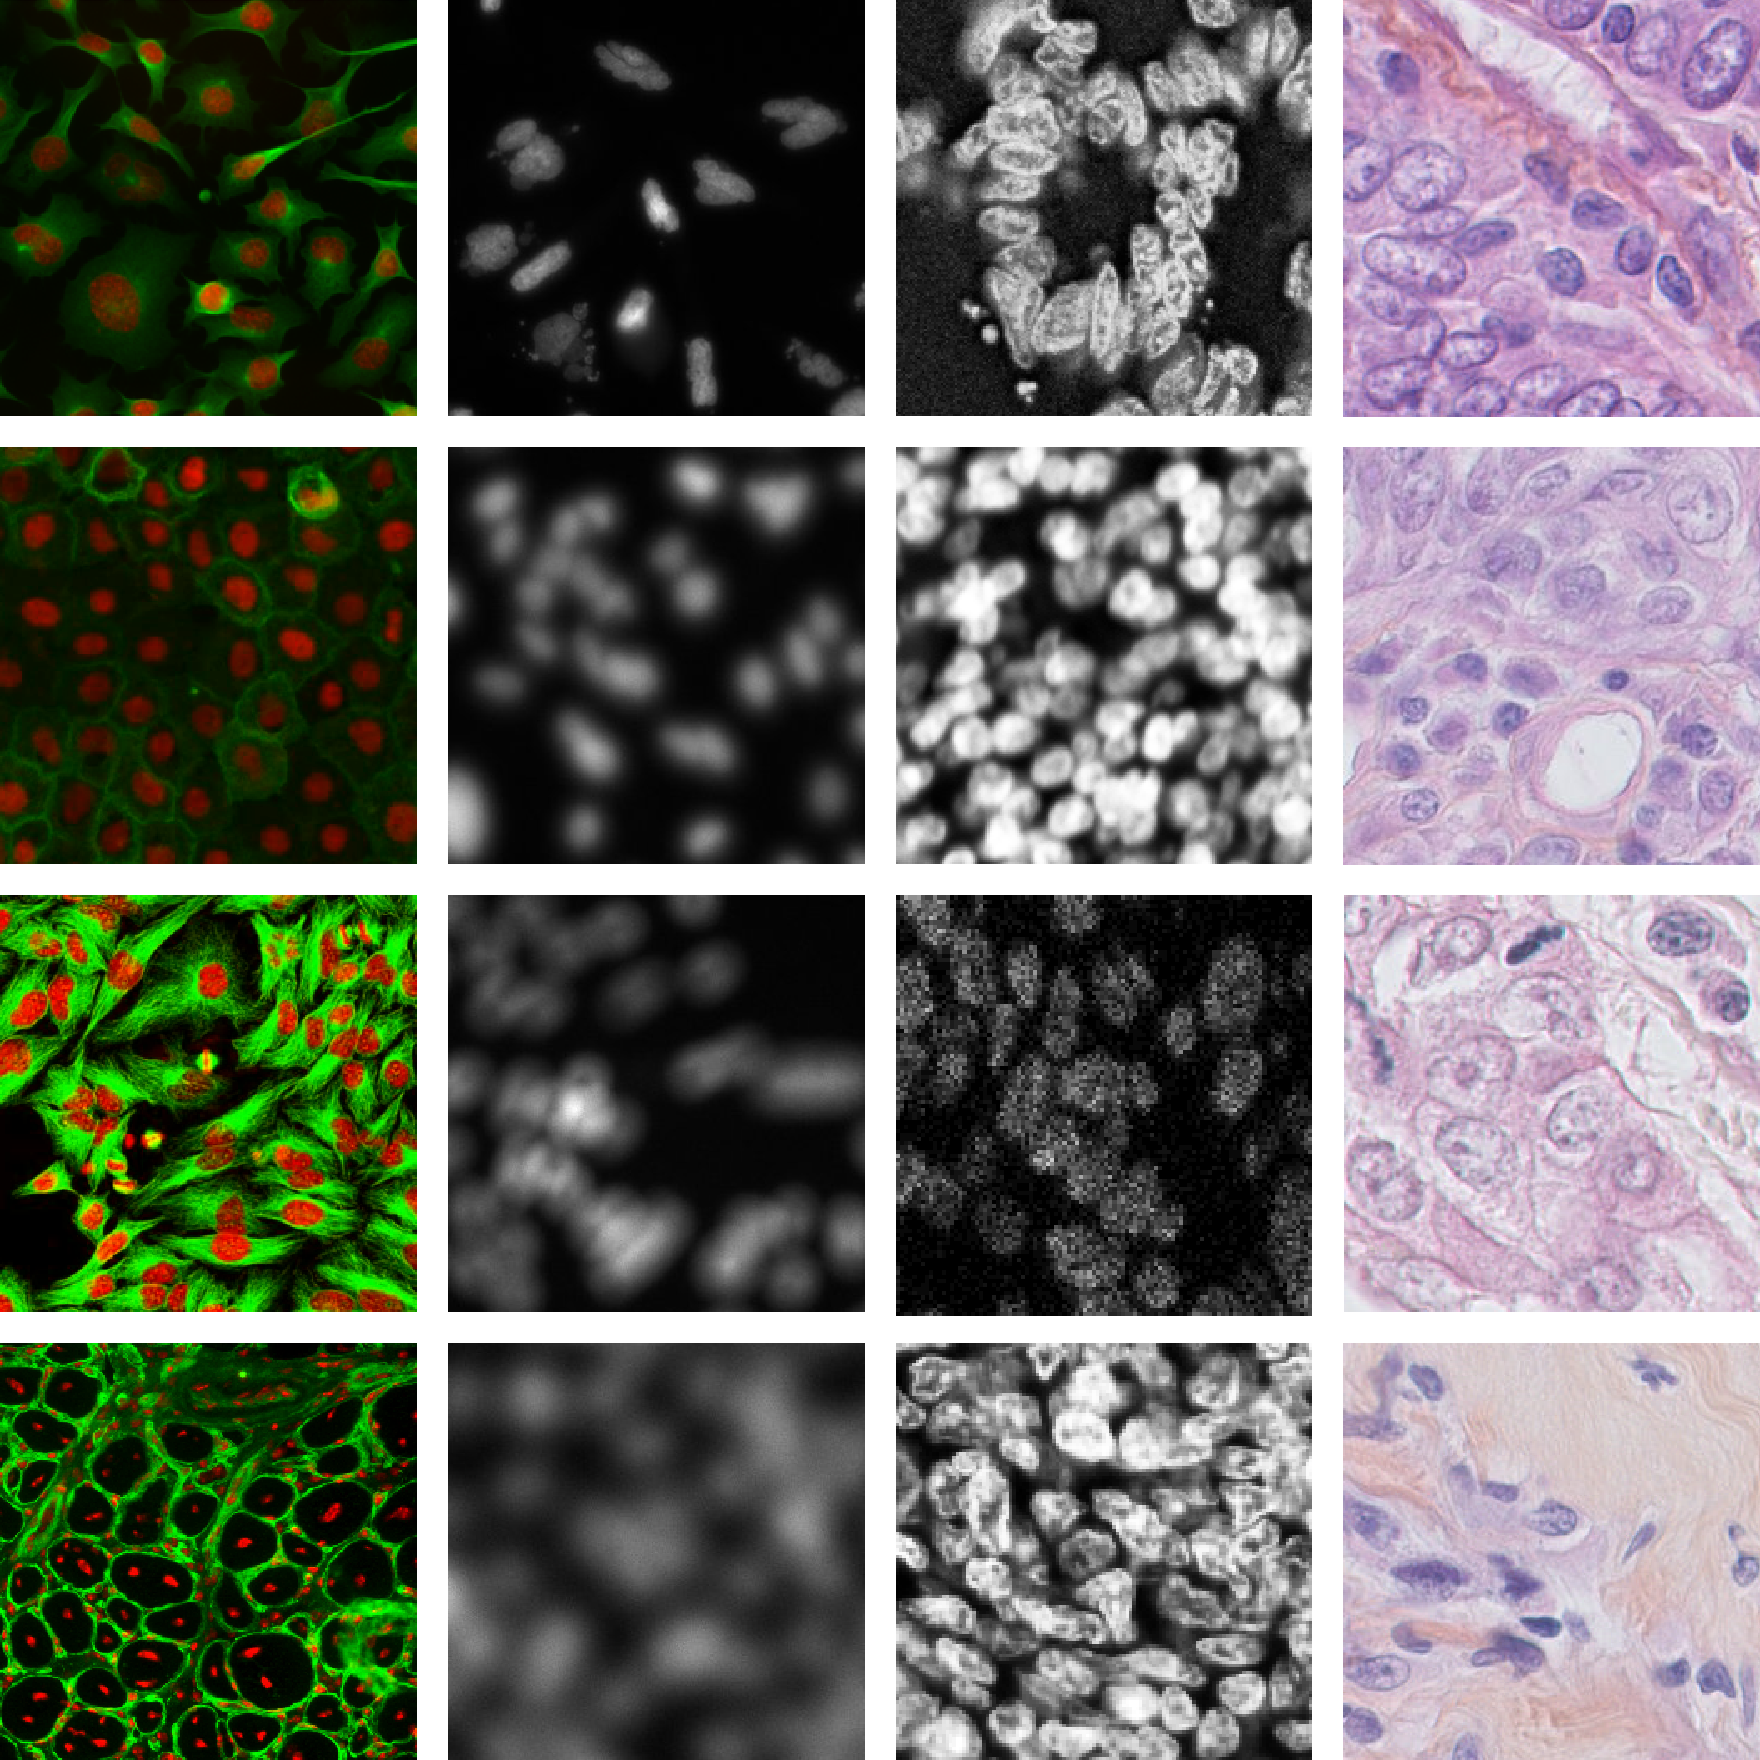
\includegraphics[width=\linewidth]{figs/Modality_Samples_4x4.pdf}
    \caption{\textbf{Illustating variability across microscopy imaging modalities and types.} First column describes images collected from Cellpose Gen. data~\cite{stringer2021cellpose}, second column represents various images of Human U20S cells with Hoechst and phalloidin stains from BBBC006~\cite{ljosa2012annotated}, the third column illustrates images from  Tissuenet~\cite{greenwald2022whole}, and the forth column shows results obtained using H \& stain from TNBC~\cite{naylor2018segmentation}.}
    \label{fig:modality}
\end{figure}


We are interested in improving tasks such as cellular activity monitoring. Various microscopes can be employed to produce videos of time-sequence observations in 2D and 3D volumes. For example, light-sheet, fluorescent, or confocal microscopy, each requiring tracking the cells in the volume they occupy. In \Cref{fig:modality}, we show different imaging data obtained using different platforms and on different tissue types. Since the variability is expanding as the cells can differ in size and shape as well as imaging modalities, there would not be a single method generalized towards all and any type of cell monitoring. \cite{bragantini2024ultrack} argues that it is merely because of the low quality segmentation algorithms which adds noise to the predictions and therefore, cannot associate cells properly for the task of lineage linking. We follow that idea, and propose to tackle the test-time adaptation problem of cell instance segmentation to improve cell tracking in this manuscript.
 
\section{Methods}

\subsection{Overview}
Our hypothesis is that performing test time adaptation on cell segmentation will improve cell tracking performance since the associations are based on simple metrics such as IoU and Euclidean distance of the centroids~\cite{bragantini2024ultrack}. In our approach, we assume to have a pre-trained network available that was trained on a source dataset. Since Cellpose~\cite{stringer2021cellpose} is still one of the state-of-the-art algorithms for the task of cell instance segmentation, we choose that to be our baseline algorithm and build TTA framework on top of that. In the following sections, we will discuss preliminaries on Cellpose~\cite{stringer2021cellpose}, TTA, and our proposed framework. 



\subsection{Cell Segmentation}

To test our hypothesis, we use one of the state-of-the-art cell instance segmentation algorithms as our segmentation framework Cellpose~\cite{stringer2021cellpose}. It is pretrained on diverse datasets and has good generalization capability. However, it is not pretrained on all imaging modalities or cell types, rendering it less useful in out-of-distribution datasets. We propose to utilize their pretrained model and perform test-time adaptation. 

Here, we describe the inner workings of Cellpose~\cite{stringer2021cellpose}: given an image $I$, the model uses a network $f$ to produce a dense, pixel-wise feature $\bm{Z} = f(I)$, where $ \bm{Z} = [Z_1, Z_2, Z_3] \in \mathbb{R}^{h \times w \times 3}$. Given the feature $\mathbf{z} = [z_1, z_2, z_3] \in \bm{Z}$ for some pixel $i$, then $\bm{z} \doteq (z_1, z_2)$ has the meaning of gradient pointing towards the center of the cell structure to which pixel $i$ belongs. Collectively, $(Z_1,Z_2)$ form a \emph{gradient flow}. Instead, $z \doteq z_3$ represents the unnormalized score indicating the probability of pixel $i$ to belong to a cell structure. Note that with this notation, the feature $\mathbf{z}$ can be written as $\mathbf{z} = [\bm{z}, z]$. The network $f$ is trained in a supervised manner with pixel-wise instance segmentation loss
\begin{equation}
  \mathcal{L}_i^{IS} = (z_1 - \mathtt{g_x})^2 + (z_2 - \mathtt{g_y})^2 + \nu H(\mathtt{m},\sigma(z))  \; ,
\end{equation}
where, for pixel $i$,  $(\mathtt{g_x}, \mathtt{g_y})$ represents the ground-truth gradient label with unit $\ell_2$-norm, $\mathtt{m} \in \{0, 1\}$ is the binary mask label indicating absence/presence of a cell structure, $\sigma(z) \doteq 1/(1+\exp(-z))$, $H$ represents the binary cross-entropy, and $\nu$ is a hyperparameter set to $0.04$. The pixel-wise loss contributions are then aggregated into a final loss $\mathcal{L}^{IS} = \sum \mathcal{L}_i^{IS}$ for the image $I$.


Given the feature $\bm{Z}$, the cell instance segmentation head $g$ produces the mask $Y = g(\bm{Z})$, where for pixel $i$, the predicted label $y$ is a number in the set $\{0, 1, \cdots, N \}$, with $N$ being the total number of cell instances segmented. Pixels belonging to the same cell instance have same label, and $y=0$ indicates absence of a cell instance. 


\subsection{Test-Time Adaptation Loss Computation}

At test-time, we follow two TTA constraints: (i) no source data available and (ii) no target labels available. In this setting, we want to perform the adaptation in a fully unsupervised manner. Once we have a pre-trained Cellpose~\cite{stringer2021cellpose} model available, we will utilize its predictions on the target data to perform the adaptation. Here,   

\subsubsection{Self-Entropy}\label{sec:tta-se}
One of our first objectives is to calculate the Shannon entropy~\cite{shannon1948mathematical} of the mask probability predictions. Shannon entropy~\cite{shannon1948mathematical} allows us to quantify the model uncertainty in the model predictions. As it refers to the uncertainty of the model, we could also utilize this information as a metric to decide which predictions are confident predictions. It is especially crucial as data distributions can change during inference. As our mask predictions are given by $\sigma(z)$, our Shannon entropy~\cite{shannon1948mathematical} becomes the following:

\begin{equation}
    \mathcal{L}_i^{SE} = -\sigma(z) \log \sigma(z) \; ,
\end{equation}

However, since our mask predictions refer to a binary crossentropy task and do not possess a probability distribution over $k$ classes, we redefine the entropy as the following:
\begin{equation}
    \mathcal{L}_i^{SE} = -(\sigma(z) \log \sigma(z) + (1-\sigma(z)) \log (1-\sigma(z))) \; ,
\end{equation}

Now that we calculated $\mathcal{L}^{SE}$ for the binary mask predictions, we can use this information to collect more confident prediction. We choose a threshold $\delta$ that describes if the $\mathcal{L}_i^{SE}$ is lower than the threshold, then the predictions are confident enough. It is given by $\hat{\bm{z}} = \bm{z}[\mathcal{L}^{SE}<\delta]$. Further, once the indices are collected, we choose a probability threshold $p$ that determines if the original predictions have large enough probability to be considered a valid prediction which is given by $\hat{\bm{z}} = \hat{\bm{z}}[\sigma(z)<p]$. Now, we have a refined set of indices which will be useful in the next section. 

\subsubsection{Contrastive Flow Loss} \label{sec:tta-cfl}
Proposed framework employs a contrastive prediction task for enhancing gradient flow features of the target pixels. \cite{keaton2023celltranspose} first proposed to utilize a contrastive objective in gradient flow alignment task and we follow their formulation in this paper; however, their framework is supervised whereas our framework performs contrastive learning in a self-supervise manner. We decide a positive sample with refined binary mask from  $\hat{z}$ with predictions $\mathbb{I}[\hat{z}>p]$, that is $\hat{z_+},\hat{z}>p$. We further decide the gradient flow features $\hat{\bm{z}}_+$ closest to a prediction  $\hat{\bm{z}} = (z_1,z_2)$ according to a similarity metric. In our case we use cosine similarity given by $s(\bm{u},\bm{v})\doteq\frac{\bm{u}^T\bm{v}}{\| \bm{u} \| \| \bm{v}\| }$, where $\| \cdot \|$ denotes $l_2$-norm.  We collect the set of negative samples $\mathcal{N}_i = \{ \hat{\bm{ z}}_- \; | \; s(\hat{\bm{ z}}_+,\hat{\bm{ z}}_-) < \theta, \hat{z}_- > p\}$, where $\theta$ is an appropriate hyperparameter threshold we choose. Once the positive and negative samples are collected, we deploy our contrastive objective for pixel $i$ that will attempt to pull the positive pairs $(\hat{\bm{z}}, \hat{\bm{z}_+})$, at the same time pushing away the negative pairs $(\hat{\bm{z}}, \hat{\bm{z}}_-)$.  \cite{wang2021understanding} suggests clever hard-mining strategies for learning with a contrastive objective in which the hard-mining of negative samples limits the need for a huge number of negative samples at the same time improving the convergence speed. Since our objective is adapting at test time, fast convergence will benefit the algorithm grately. Therefore, in our case, similar to \cite{keaton2023celltranspose}, we follow hard-mining sampling strategy for negative samples. In essence, $\mathcal{N}_i$ is composed of a set if pixels that are close to the positive samples. Please refer to  \cite{keaton2023celltranspose} for the details. \\

Given a batch of target image patches, each patch is paired with another patch from the same batch. We then compute the contrastive flow loss aggregating all the components coming from the all the valid pixels, i.e.,  $\hat{z}_- > p$. 
Now the loss function becomes the following:

\begin{equation}
    \small
    \mathcal{L}_i^{CF} = - \log \frac{\exp( s (\hat{\bm{ z}}, \hat{\bm{ z}}_+)/\tau )}{ \exp( s (\hat{\bm{ z}}, \hat{\bm{ z}}_+)/\tau ) + \sum_{\hat{\bm{ z}}_- \in \mathcal{N}_i} \exp( s (\hat{\bm{ z}}, \hat{\bm{ z}}_-)/\tau ) }\\
    \label{eq-contrastive-flow-loss}
  \end{equation}
where $\tau$ refers to a temperature parameter we choose. 

\subsubsection{Adaptation Loss}
In \cref{sec:tta-se}, we calculate self-entropy for the binary mask predictions and in \Cref{sec:tta-cfl}, we calculate a contrastive object to enhance the gradient flow estimations. We combine this two losses for the model update at test time as shown below:
\begin{equation}
    \small
    \mathcal{L}^{TTA} = \lambda_1\frac{1}{| \mathcal{M}_1 |} \sum_{\mathcal{M}_{1}} \mathcal{L}^{SE}_i + \lambda_2\frac{1}{| \mathcal{M}_2 |} \sum_{\mathcal{M}_2} \mathcal{L}^{CF}_i \; .
    \label{eq-tta-loss}
  \end{equation}
Where, total pixel belonging to the target patch, we define it by $\mathcal{M}_1$, and the valid pixels we define that set by $\mathcal{M}_2$. $\lambda_1$ and $\lambda_2$ are the weight parameters for the loss. This combination of losses is used to perform the adaptation. In the next section, we will discuss what parameters we want to update during TTA. 

\subsection{Test-Time Adaptation Parameter Updates}
Studies have shown that the major cause of performance degradation in convolution-based networks is the shift in batch-normalization statistics during inference~\cite{wang2020tent,niu2022efficient,zaveri2025improving,li2016revisiting,mirza2022norm,pan2018two,schneider2020improving}. We take advantage of these findings and propose to only update the batch-normalization parameters. They are calculated by the following equations:
\begin{equation}\small
    \centering
    \label{eq:bn}
        \begin{aligned}  
        BN(x) = \gamma \frac{x - E(x)}{\sqrt{Var(x)}} +  \beta ,
        \end{aligned}
\end{equation}
\begin{equation}\small
    \centering
    \label{eq:bn_running}
        \begin{aligned}  
            \overline{\mu}_t = (1-\alpha)  \overline{\mu}_{t-1} +  \alpha  {\mu}_t ,\\
            \overline{\sigma}_{t}^2 = (1-\alpha) \overline{\sigma}_{t-1}^2 +  \alpha {\sigma}_{t}^2 ,
        \end{aligned}
\end{equation}

where $x$ is the input feature, $E(x)$ and $Var(x)$ are the expected value and variance of $x$. $\gamma$ and $\beta$ are learnable parameters for scaling and shifting. The BN layers keep track of the running mean and variance through Equation \ref{eq:bn_running}, where ${\mu}_t$ and ${\sigma}_{t}$ are current expected value and variance respectively, and $\overline{\mu}_t$ and $\overline{\sigma}_{t}$ are used for $E(x)$ and $Var(x)$, respectively. $\alpha$ is the momentum parameter. We propose to estimate the learnable parameters $\gamma$ and $\beta$ during testing that requires a backward pass. Additionally, we also dynamically updates the BN statistics $E(x)$ and $Var(x)$ during testing according to the following strategy:
\begin{equation}
  \centering
  \label{eq:bn_update}
      \begin{aligned}  
          \overline{\mu}_{I,t} &= (1-\lambda{_{BN}}) \overline{\mu} +  \lambda{_{BN}} \mu_{I,t} \; ,\\
          \overline{\sigma}_{I,t}^2 &= (1-\lambda{_{BN}}) \overline{\sigma}^2 +  \lambda{_{BN}} \sigma_{I,t}^2 \; ,
      \end{aligned}
\end{equation}
where $\overline{\mu}$ and $\overline{\sigma}^2$ are the final running mean and variance of the model trained on the source data, respectively, and $\mu_{I,t}$, and $\sigma_{I,t}^2$ are mean and variance calculated from the instance at time $t$, respectively. $\overline{\mu}_{I,t}$ and $\overline{\sigma}_{I,t}^2$ are updated based on the current instance and used for feature normalization at time $t$. $ \lambda{_{BN}}$ is set to 0.1. 
